\documentclass[aps,prb,twocolumn,superscriptaddress,floatfix,longbibliography]{revtex4-2}

\usepackage[utf8]{inputenc}
\usepackage[spanish]{babel}
\usepackage{graphicx}
\usepackage{amsmath}
\usepackage{subcaption}
\usepackage{wrapfig} 
\usepackage[export]{adjustbox}

\usepackage{amsmath,amssymb} % math symbols
\usepackage{bm} % bold math font
\usepackage{graphicx} % for figures
\usepackage{comment} % allows block comments
\usepackage{textcomp} % This package is just to give the text quote '
%\usepackage{ulem} % allows strikeout text, e.g. \sout{text}

\usepackage[spanish]{babel}

\usepackage{enumitem}
\setlist{noitemsep,leftmargin=*,topsep=0pt,parsep=0pt}

\usepackage{xcolor} % \textcolor{red}{text} will be red for notes
\definecolor{lightgray}{gray}{0.6}
\definecolor{medgray}{gray}{0.4}

\usepackage{hyperref}
\hypersetup{
colorlinks=true,
urlcolor= blue,
citecolor=blue,
linkcolor= blue,
bookmarks=true,
bookmarksopen=false,
}

% Code to add paragraph numbers and titles
\newif\ifptitle
\newif\ifpnumber
\newcounter{para}
\newcommand\ptitle[1]{\par\refstepcounter{para}
{\ifpnumber{\noindent\textcolor{lightgray}{\textbf{\thepara}}\indent}\fi}
{\ifptitle{\textbf{[{#1}]}}\fi}}
%\ptitletrue  % comment this line to hide paragraph titles
%\pnumbertrue  % comment this line to hide paragraph numbers

% minimum font size for figures
\newcommand{\minfont}{6}

% Uncomment this line if you prefer your vectors to appear as bold letters.
% By default they will appear with arrows over them.
% \renewcommand{\vec}[1]{\bm{#1}}

%Cambiar Cuadros por Tablas y lista de...
%\renewcommand{\listtablename}{Índice de tablas}
\renewcommand{\tablename}{Tabla}
\renewcommand{\date}{Fecha}

\graphicspath{ {C:/Users/lupam/Mi unidad/Pablo Chehade/Instituto Balseiro (IB)/Métodos numéricos en fluidos I/Metodos_Num_Fluidos_I/Guias/Guia_1/Informe/Figures} } %Para importar imágenes desde una carpeta


\usepackage[bottom]{footmisc} %para que las notas al pie aparezcan en la misma página



\begin{comment}

%Comandos de interés:

* Para ordenar el documento:
\section{Introducción}
\section{\label{sec:Formatting}Formatting} %label para luego hacer referencia a esa sección

\ptitle{Start writing while you experiment} %pone nombre y título al documento dependiendo de si en el header están los comandos \ptitletrue y \pnumbertrue

* Ecuaciones:
\begin{equation}
a^2+b^2=c^2 \,.
\label{eqn:Pythagoras}
\end{equation}

* Conjunto de ecuaciones:
\begin{eqnarray}
\label{eqn:diagonal}
\nonumber d & = & \sqrt{a^2 + b^2 + c^2} \\
& = & \sqrt{3^2+4^2+12^2} = 13
\end{eqnarray}

* Para hacer items / enumerar:
\begin{enumerate}
  \item
\end{enumerate}

\begin{itemize}
  \item
\end{itemize}

* Figuras:
\begin{figure}[h]
    \includegraphics[clip=true,width=\columnwidth]{pixel-compare}
    \caption{}
     \label{fig:pixels}
\end{figure}

* Conjunto de figuras:
(no recuerdo)


* Para hacer referencias a fórmulas, tablas, secciones, ... dentro del documento:
\ref{tab:spacing}

* Para citar
Elementos de .bib
\cite{WhitesidesAdvMat2004}
url
\url{http://www.mendeley.com/}\\

* Agradecimientos:
\begin{acknowledgments}
We acknowledge advice from Jessie Zhang and Harry Pirie to produce Fig.\ \ref{fig:pixels}.
\end{acknowledgments}

* Apéndice:
\appendix
\section{\label{app:Mendeley}Mendeley}

* Bibliografía:
\bibliography{Hoffman-example-paper}

\end{comment}



\begin{document}

% Allows to rewrite the same title in the supplement
\newcommand{\mytitle}{Laboratorio 1 - Diferencias finitas}

\title{\mytitle}

\author{Pablo Chehade \\
    \small \textit{pablo.chehade@ib.edu.ar} \\
    \small \textit{Métodos Numéricos en Fluidos I, Instituto Balseiro, CNEA-UNCuyo, Bariloche, Argentina, 2022} \\}


\begin{abstract}

Se estudió el comportamiento de distintas aproximaciones numéricas en un problema de valores de contorno tipo Dirichlet de solución exacta conocida. Se empleó el método de diferencias finitas centradas de orden 2 y la aproximación de Padé de orden 4. En primer lugar, se analizó cualitativamente ambas aproximaciones para $K$ y $N$ fijos. Se observó que la aproximación de Padé es más precisa que la de diferencias centradas. En segundo lugar, se estudió la dependencia del error en un punto particular en función del espaciamiento $h$. En ambos métodos, el error disminuye a medida que $h$ también lo hace, con distinto ritmo para cada aproximación. Finalmente, se estudió la capacidad de ambos métodos para adaptarse a soluciones oscilatorias. En concreto, se calculó cuántos puntos discretos $\mathrm{N_{min}}$ son necesarios para obtener un error total menor a una tolerancia determinada en función de las oscilaciones de la solución exacta. Se obtuvo que en la aproximación de Padé se necesitan menos puntos que en la de diferencias centradas para obtener el mismo error total, independientemente de la frecuencia de las oscilaciones y de la norma elegida para calcular el error.

\end{abstract}

\maketitle

\section{Introducción}
\ptitle{En física, no todos los problemas tienen solución analítica, muchas veces es necesario recurrir a aproximaciones}

En ciencias físicas no todos los problemas tienen solución analítica \cite{Chule}. Debido a esto, es necesario recurrir a aproximaciones del mismo que sí posean solución o a esquemas numéricos que permitan aproximarlo computacionalmente. Sin embargo, estos esquemas no están excentos de error, por lo que deben ser estudiados en detalle para determinar su validez y aplicabilidad. Para esto es útil aplicar estos esquemas a problemas de solución exacta conocida.

\ptitle{En este trabajo se estudió el comportamiento de distintas aproximaciones numéricas en el siguiente problema de valores de contorno tipo Dirichlet}

En este trabajo se estudió el comportamiento de distintas aproximaciones numéricas en el siguiente problema de valores de contorno tipo Dirichlet
\begin{equation}
    \left\{\begin{matrix}
        \frac{d^2 y}{dx^2} - y = g(x), \\ 
        g (x) = - \sum_{j = 1}^K (1 + (j \pi)^2)\sin{(j \pi x)}, 0 \leq x \leq 1,\\
        y(0) = 0,\\
        y(1) = 1, \\
        \end{matrix}\right.
    \label{ec:PVC}
\end{equation}

con solución analítica
\begin{equation}
    y(x) = \frac{e^x - e^{-x}}{e - e^{-1}} + \sum_{j = 1}^K \sin{(j \pi x)}
    \label{ec:sol_analitica}
\end{equation}

\section{Método Numérico}

\ptitle{Discretización del dominio}

Para resolver numéricamente el problema de valores de contorno es necesario discretizar el dominio y proponer un esquema numérico que permita obtener la solución aproximada. El dominio se discretizó con puntos equiespaciados $x_i = i h$ donde $i = 1,\cdots, N$ y $h = 1/(N+1)$. En base a esto, el problema de valores iniciales \ref{ec:PVC} se puede escribir como
\begin{equation}
    \left\{\begin{matrix}
        y_i'' - y_i = g_i, i = 1, \cdots, N\\
        y_0 = y(0) = 0,\\
        y_{N+1} = y(1) = 1, \\
        \end{matrix}\right.
    \label{ec:PVC_numerico}
\end{equation}
donde $y_i''= \frac{d^2 y_i}{dx^2}$ y $g_i = g(x_i)$.

\ptitle{Para estimar y'' emplearon diferencias finitas centradas de segundo orden y el \textcolor{red}{esquema} de Padé \textcolor{red}{de 4to orden}}
Para estimar $y_i''$ se pueden utilizar distintos esquemas numéricos. En este trabajo se emplearon diferencias finitas centradas y la aproximación de Padé.


\subsection{Diferencias finitas centradas}
La fórmula de diferencias finitas centradas de segundo orden para la derivada segunda es \cite{Moin}
\begin{equation}
    y_i'' = \frac{y_{i+1} - 2 y_i + y_{i-1}}{h^2} + O(h^2).
    \label{ec:diferencias_centradas}
\end{equation}
Aplicándola a la ecuación diferencial \ref{ec:PVC_numerico} para los nodos internos $i = 2, \cdots, N-2$, se obtiene
\[ \frac{1}{h^2} y_{i-1} + \left (-\frac{2}{h^2} - 1 \right ) y_i + \frac{1}{h^2} y_{i-1} = g_i.\]
Para los nodos del borde se puede emplear la misma aproximación bajo la consideración de que $y_0 = y(0)$ e $y_{N+1} = y(1)$, es decir,
\[\frac{1}{h^2}y_2 + \left (-\frac{2}{h^2} - 1 \right ) y_1 = g_1 - \frac{1}{h^2}y(0)  \]
\[\frac{1}{h^2}y_N + \left (-\frac{2}{h^2} - 1 \right ) y_{N-1} = g_N - \frac{1}{h^2}y(1)  \]
El sistema de ecuaciones algebraicas anterior se puede escribir de la forma lineal $A_{DC} \vec{y} = \vec{b}$, donde
\[
    A_{DC} = \frac{-1}{h^2}\left(\begin{matrix}
        2 + h^2 & -1 & 0 & \cdots & 0 & 0\\
        -1 & 2 + h^2 & -1 & \cdots & 0 & 0\\
        0 & -1 & 2 + h^2 & \cdots & 0 & 0\\
        \vdots & \vdots & \vdots & \ddots & \vdots & \vdots\\
        0 & 0 & 0 & \cdots & 2 + h^2 & -1\\
        0 & 0 & 0 & \cdots & -1 & 2 + h^2\\
        \end{matrix}\right),
\]
\[\vec{y} = (y_1, y_2, \cdots, y_N)^T \, \mathrm{y}\]
\[\vec{b} = (g_1 - y(0)/h^2, g_2, \cdots, g_{N-1}, g_N -  y(1)/h^2)^T\]




\subsection{Aproximación de Padé}

\ptitle{Obtención del sistema lineal en los nodos internos}
La fórmula de Padé de 4to orden para la derivada segunda es \cite{Moin}
\begin{equation}
    \frac{1}{12} y_{i-1}'' + \frac{10}{12} y_i'' + \frac{1}{12} y_{i+1}'' = \frac{y_{i+1} - 2 y_i + y_{i-1}}{h^2} + O(h^4)
    \label{ec:Pade_interior}
\end{equation}
válida sólo para los nodos internos $i = 2, \cdots, N-2$.

\ptitle{Obtención del sistema lineal en el borde izquierdo}
Por otro lado, para los nodos del borde con $i = 1$ e $i = N$ es necesario derivar una aproximación de Padé. Para esto basta plantear
\begin{equation}
    y_1'' + b_2 y_2'' = a_0 y_0 + a_1 y_1 + a_2 y_2 +O(h^\alpha)
    \label{ec:Pade_izq_gral}
\end{equation}
y determinar los coeficientes $a_0$, $a_1$, $a_2$ y $b_2$ de modo de obtener el mayor orden de aproximación $\alpha$ posible. Para esto se desarrolla en Taylor $y_2''$, $y_0$ e $y_2$ alrededor de $x_1$. De este modo,
\begin{eqnarray}
    \nonumber y_2'' & = & y_1'' + h y_1''' + \frac{h^2}{2} y_1^{(IV)} + O(h^3), \\ 
    \nonumber y_2 & = & y_1 + h y_1' + \frac{h^2}{2} y_1'' + \frac{h^3}{6}y_1''' + \frac{h^4}{24} y_1^{(IV)} + O(h^3), \\
    \nonumber y_0 & = & y_1 - h y_1' + \frac{h^2}{2} y_1'' - \frac{h^3}{6}y_1''' + \frac{h^4}{24} y_1^{(IV)} + O(h^3),
\end{eqnarray}
donde se consideró que $a_2$ tiene unidades de $1/h^2$. Reemplazando estas expresiones en \ref{ec:Pade_izq} se obtiene
\begin{eqnarray}
    \nonumber y_1'' & = & y_1( a_0 + a_1 + a_2) + y_1'(-a_0 h + a_2 h) \\ 
    \nonumber & + & y_1''(a_0 \frac{h^2}{2} + a_2 \frac{h^2}{2} - b_2) + y_1'''(- a_0 \frac{h^3}{6} + a_2 \frac{h^3}{6} - b_2 h) \\
    \nonumber & + & y_1^{(IV)}(a_0 \frac{h^4}{24} + a_2 \frac{h^4}{24} - b_2 \frac{h^2}{2} ) + O(h^3).
\end{eqnarray}
Igualando ambos miembros da lugar al siguiente conjunto de ecuaciones para los coeficientes $a_0$, $a_1$, $a_2$ y $b_2$
\[\left\{\begin{matrix}
    a_0 + a_1 + a_2 = 0 \\
    h(-a_0 + a_2) = 0 \\
    a_0 \frac{h^2}{2} + a_2 \frac{h^2}{2} - b_2 = 1\\
    h(- a_0 \frac{h^2}{6} + a_2 \frac{h^2}{6} - b_2) = 0 \\
    \frac{h^2}{2}(a_0 \frac{h^2}{12} + a_2 \frac{h^2}{12} - b_2) = 0
    \end{matrix}\right.
\]
Solo es posible cumplir las cuatro primeras ecuaciones mediante la elección  $a_0 = 1/h^2$, $a_1 = -2/h^2$, $a_2 = 1/h^2$ y $b_2 = 0$. Al no ser posible anular el término de orden $h^2$, la aproximación de Padé resultante es de segundo orden. La expresión final es
\begin{equation}
    y_1'' = \frac{y_{2} - 2 y_1 + y_{0}}{h^2} + O(h^2).
    \label{eq:Pade_izq}
\end{equation}
que coincide con diferencias centradas de orden dos \ref{ec:diferencias_centradas}.

\ptitle{Obtención del sistema lineal en el borde derecho}
Análogamente, se puede repetir el procedimiento para el nodo de borde $i = N$. Planteando
\[y_N'' + b_{N-1} y_{N-1}'' = a_{N-1} y_{N-1} + a_N y_N + a_{N+1} y_{N+1} +O(h^\alpha)\]
y desarrollando en Taylor $y_{N-1}''$, $y_{N-1}$ e $y_{N+1}$ alrededor de $x_N$, se obtiene un sistema de ecuaciones para los coeficientes. La aproximación de Padé resultante es de segundo orden y su expresión es
\begin{equation}
    y_N'' = \frac{y_{N+1} - 2 y_N + y_{N-1}}{h^2} + O(h^2),
    \label{eq:Pade_der}
\end{equation}
idéntica a la de diferencias centradas de orden dos \ref{ec:diferencias_centradas}.

\ptitle{Obtención del sistema lineal}
Empleando las fórmulas de diferencia finita de Padé de segundo orden (\ref{eq:Pade_izq}, \ref{eq:Pade_der} y \ref{ec:Pade_interior}) se puede escribir la relación lineal $A_P \vec{y''} = B_P \vec{y} + \vec{c}$, donde
\begin{equation}
    A_P = \left(\begin{matrix}
    1 & 0 & 0 & \cdots & 0 & 0 & 0 \\
    \frac{1}{12} & \frac{10}{12} & \frac{1}{12} & \cdots & 0 & 0 & 0 \\
    0 & \frac{1}{12} & \frac{10}{12} & \cdots & 0 & 0 & 0 \\
    \vdots & \vdots & \vdots & \ddots & \vdots & \vdots & \vdots \\
    0 & 0 & 0 & \cdots & \frac{10}{12} & \frac{1}{12} & 0 \\
    0 & 0 & 0 & \cdots & \frac{1}{12} & \frac{10}{12} & \frac{1}{12} \\
    0 & 0 & 0 & \cdots & 0 & 0 & 1
    \end{matrix}\right)
\end{equation}
\begin{equation}
    B_P = \frac{1}{h^2} \left(\begin{matrix}
    -2 & 1 & 0 & \cdots & 0 & 0 & 0 \\
    1 & -2 & 1 & \cdots & 0 & 0 & 0 \\
    0 & 1 & -2 & \cdots & 0 & 0 & 0 \\
    \vdots & \vdots & \vdots & \ddots & \vdots & \vdots & \vdots \\
    0 & 0 & 0 & \cdots & -2 & 1 & 0 \\
    0 & 0 & 0 & \cdots & 1 & -2 & 1 \\
    0 & 0 & 0 & \cdots & 0 & 1 & -2
    \end{matrix}\right)
\end{equation}
ambas matrices tridiagonales. Mientras que
$\vec{y''} = (y_1'', y_2'', \cdots, y_N'')^T,$
$\vec{y} = (y_1, y_2, \cdots, y_N)^T$
y
$\vec{c} = (y(0)/h^2, 0, \cdots, 0, y(1)/h^2)^T$

Aplicando esta relación lineal a la ecuación diferencial \ref{ec:PVC_numerico} se obtiene el sistema lineal
\[(B_P - A_P)\vec{y} = A_P\vec{g} - \vec{c}\]
donde $\vec{g} = (g_1, g_2, \cdots, g_N)$. 


\ptitle{Resumen de los que se tratará en Resultados}
Habiendo desarrollado ambos métodos y habiéndolos aplicado a la ecuación diferencial, se está en condiciones de resolver el problema y comparar con la solución exacta.


\section{Resultados}

\begin{figure}[h]
    \includegraphics[clip=true,width=\columnwidth]{Figures/comportamiento_cuali.eps}
    \caption{Solución exacta y soluciones aproximadas en puntos discretos por los métodos de diferencias finitas centradas y aproximación de Padé para $K = 6$ y $N = 23$.}
     \label{fig:comportamiento_cuali}
\end{figure}

\ptitle{Comportamiento cualitativo}
Se analizaron cualitativamente ambas aproximaciones para $K=6$ y $N=23$ fijos. En la figura \ref{fig:comportamiento_cuali} se grafica la solución exacta junto a las soluciones aproximadas en puntos discretos obtenidas mediante ambos métodos. A grandes rasgos se observa que si bien ambos logran aproximar la solución, el método de diferencias centradas tiene mayor error que la aproximación de Padé, especialmente en los puntos máximos y mínimos de la oscilación. Para analizar cuantitativamente la diferencia se calculó el error local en el punto central $x = 0.5$ en función del espaciamiento $h$. Esta dependencia se grafica en la figura \ref{fig:error_local_0.5} en escala log-log. Se observa una dependencia similar para ambos métodos. Inicialmente, para $h$ grande, el error presenta un comportamiento aleatorio. A medida que $h$ disminuye, el error varía como una potencia de $h$, es decir, de forma lineal en escala logarítmica. Por último, para valores de $h$ menores, el error aumenta debido a los errores de precisión de la computadora. En base a la dependencia observada en la zona intermedia se ajustó una recta en escala log-log, es decir, la función $\mathrm{log(error)} = a \mathrm{log(h)} + b$ con $a$ pendiente y $b$ ordenada al origen. De este modo $a$ representa el orden del error de truncamiento. Para diferencias finitas centradas se obtuvo un orden $a_{DC} = 1.995 \pm 0.004$. Esto es consistente con el orden de aproximación de orden 2 del método numérico, tal como se observa en \ref{ec:diferencias_centradas}. Por otro lado, para la aproximación de Padé se obtuvo un orden $a_P = 4.47 \pm 0.07$. Como en los nodos del borde el orden de aproximación es 2 y en los nodos internos el orden es 4, se hubiera esperado que el orden de aproximación en el punto central se encuentre entre 2 y 4. Este no es el caso y habría que estudiar con mayor detalle a qué se debe este comportamiento.

\begin{figure}[h]
    \includegraphics[clip=true,width=\columnwidth]{Figures/error_local_0.5.eps}
    \caption{Error local en el punto $x = 0.5$ en función del espaciamiento $h$ para diferencias finitas centradas y aproximación de Padé en escala log-log. Se ajustó en ambos casos una dependencia lineal $a \mathrm{log(h)} + b$. En el caso de diferencias finitas se obtuvo una pendiente $a_{DC} = 1.995 \pm 0.004 $ y una ordenada al origen $b_{DC} = 1.13 \pm 0.02$. Mientras que en la aproximación de Padé, $a_P = 4.47 \pm 0.07$ y $b_P = 3.9 \pm 0.2$.}
     \label{fig:error_local_0.5}
\end{figure}

\ptitle{Se determinó el nro de puntos mínimos necesarios para obtener un error menor a $10e-1$ en distintas normas en función de la frecuencia K}

\begin{table}[]
    \begin{tabular}{|l|l|l|l|l|}
    \hline
    \multicolumn{1}{|c|}{K$\textbackslash \mathrm{N_{min}}$} & \multicolumn{1}{c|}{\begin{tabular}[c]{@{}c@{}}DC\\ norma 2\end{tabular}} & \multicolumn{1}{c|}{\begin{tabular}[c]{@{}c@{}}Padé\\ norma 2\end{tabular}} & \multicolumn{1}{c|}{\begin{tabular}[c]{@{}c@{}}DC\\ norma $\infty$\end{tabular}} & \multicolumn{1}{c|}{\begin{tabular}[c]{@{}c@{}}Padé\\ norma $\infty$\end{tabular}} \\ \hline
    3 & 14 & 10 & 10 & 8 \\ \hline
    8 & 66 & 32 & 39 & 26 \\ \hline
    16 & 202 & 81 & 107 & 59 \\ \hline
    32 & 626 & 204 & 295 & 136 \\ \hline
    64 & 1962 & 514 & 826 & 314 \\ \hline
    128 & 6188 & 1294 & 2322 & 724 \\ \hline
    \end{tabular}
    \caption{\label{tab:NvsK}Número de puntos mínimos necesarios para obtener un error menor a $0.1$ en norma 2 y norma infinito en función de la frecuencia $K$ para el método de diferencias centradas (DC) y la aproximación de Padé.}
\end{table}

\begin{figure}[h]
    \includegraphics[clip=true,width=\columnwidth]{Figures/NvsK.eps}
    \caption{Número de puntos mínimos $\mathrm{N_{min}}$ necesarios para obtener un error menor a $0.1$ en función de la frecuencia $K$ para diferencias finitas centradas y aproximación de Padé en escala log-log. El error fue calculado en norma 2 y norma infinito.}
     \label{fig:NvsK}
\end{figure}

Por último, se analizó la capacidad de cada método para adaptarse a soluciones oscilatorias. Las oscilaciones están caracterizadas en este problema mediante el parámetro $K$. A mayor $K$, la solución exacta contiene componentes con mayor frecuencia, tal como se verifica en la ecuación \ref{ec:sol_analitica}. De este modo, se determinó para ambos métodos el número de puntos mínimos $\mathrm{N_{min}}$ necesarios para obtener un error total menor a $0.1$ en función del parámetro $K$. El error fue calculado en norma 2 y norma infinito. Los resultados se resumen en la tabla \ref{tab:NvsK} y se grafican en escala log-log en la figura \ref{fig:NvsK}. Como se observa $\mathrm{N_{min}}$ crece con $K$, es decir, frente a oscilaciones de mayor frecuencia son necesarios más puntos para mantener el mismo error. Sin embargo, independientemente de la norma, se necesitan más puntos en diferencias centradas que en la aproximación de Padé. Esto se debe a que esta útlima aproximación es de mayor orden que el método de diferencias centradas. Además, en ambos casos se necesitan menos puntos cuando el error se calcula en norma infinito que en norma 2. Esto se debe a que en esta última se suman cuadráticamente los errores en todos los puntos, mientras que en norma infinito solo se considera el máximo de los errores en todos los puntos. En base a esto, a igual $\mathrm{N_{min}}$ se obtendría menor error en norma infinito que en norma 2. Análogamente, a igual error, se necesitarían más puntos en norma 2 que en norma infinito.

\section{Conclusión}

Se estudió el comportamiento de distintas aproximaciones numéricas en el siguiente problema de valores de contorno tipo Dirichlet con solución exacta conocida
\begin{equation}
    \left\{\begin{matrix}
        \frac{d^2 y}{dx^2} - y = g(x), \\ 
        g (x) = - \sum_{j = 1}^K (1 + (j \pi)^2)\sin{(j \pi x)}, 0 \leq x \leq 1,\\
        y(0) = 0,\\
        y(1) = 1, \\
        \end{matrix}\right.
\end{equation}

Para los nodos internos se emplearon el método de diferencias finitas centradas de orden 2 y la aproximación de Padé de orden 4. Mientras que en los nodos del borde se emplearon diferencias finitas centradas.

En primer lugar, se analizó cualitativamente ambas aproximaciones para $K = 6$ y $N = 23$ fijos. Se observó que la aproximación de Padé es más precisa que la de diferencias centradas. En segundo lugar, con el objetivo de fundamentar cuantitativamente la afirmación anterior, se estudió la dependencia del error en el punto central en función del espaciamiento $h$. Para diferencias centradas el error disminuye con orden $1.995 \pm 0.004$, mientras que para la aproximación de Padé, con orden $ 4.47 \pm 0.07$. Finalmente, se estudió la capacidad de ambos métodos para adaptarse a las oscilaciones, representadas en este problema por el parámetro $K$ en la ecuación diferencial. Con tal fin, se calculó cuántos puntos discretos $\mathrm{N_{min}}$ son necesarios para obtener un error total menor a $0.1$ en función de $K$. El error se calculó en norma 2 y norma infinito. Se obtuvo que en la aproximación de Padé se necesitan menos puntos que en la de diferencias centradas para obtener el mismo error total, independientemente de la frecuencia de las oscilaciones y de la norma utilizada.

\bibliography{Chehade_guia1.bib}

\end{document}





